% Syntax template only; replace all content using source-derived constraints.
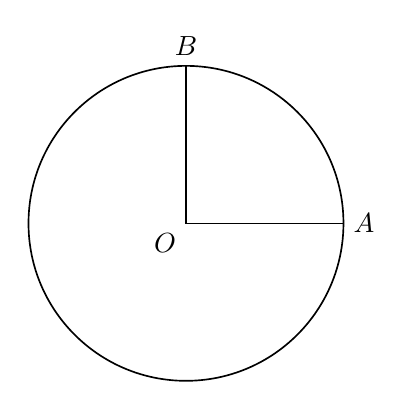
\begin{tikzpicture}[x=1cm,y=1cm,line width=.6pt,font=\normalsize]
\coordinate (O) at (0,0);
\coordinate (A) at (2,0);
\coordinate (B) at (0,2);
\draw (O) circle[radius=2cm];
\draw (A)--(O)--(B);
\node[below left] at (O) {$O$};
\node[right] at (A) {$A$};
\node[above] at (B) {$B$};
% For an original arc: \draw (A) arc[start angle=0,end angle=90,radius=2cm];
% Do not add this template's point names, circle, radii or angle to a source.
\end{tikzpicture}
